\section{The \sysname Key-Value Store}
\label{sec:store}

In this section we realise a distributed and consistent key-value store that fulfils the required properties for the \sysname protocol without the need for a consensus protocol.

\nico{TODO, go through this section and fix language and references to make sense in the new structure}

\subsection{Read and Write Protocol} \label{sec:read-write}
\Cref{fig:arke-store} presents an overview of the protocol allowing user $A$ to respectively write and read the key-value pairs $(\key_{AB}, \val_{AB})$ and $(\key_{BA}, \val_{BA})$ from the store.

\begin{figure*}[t]
    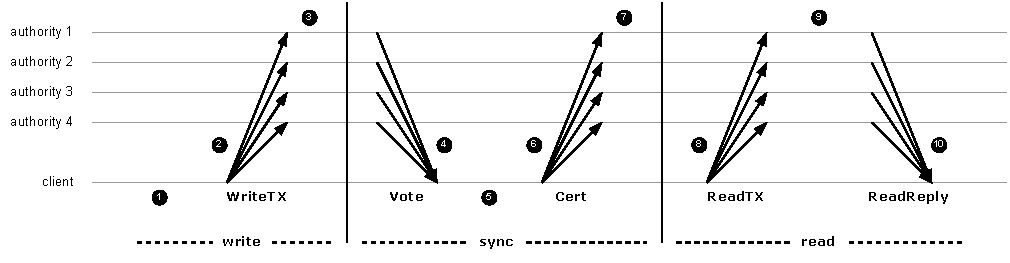
\includegraphics[width=\textwidth]{figures/arke-store.drawio.pdf}
    \caption{Example of \sysname write (\one-\three), sync (\four-\seven), and read (\eight-\ten) protocol with 4 authorities.}
    \Description{}
    \label{fig:arke-store}
\end{figure*}

\paragraph{Writing the store}
Steps \one-\three of \Cref{fig:arke-store} illustrate the high-level interactions between user $A$ and the storage authorities to allow the user to write the distributed store.
%
User $A$ uses its writing tag $t_{AB}$ (\Cref{sec:key-derivation}) as a private signing key to create and sign a \emph{write transaction}. This transaction mutates (or creates) the key-value pair $(\key_{BA}, \val_{BA}) = (g_1^{t_{BA}}, c_{BA})$ of the \sysname store~(\one).
%
The user transaction is then sent to each \sysname storage authority~(\two).
%
The authorities check it for validity and lock the store entry to mutate~(\three). The write operation is completed as soon as $2f+1$ authorities successfully terminate this step. \Cref{alg:process-tx} of \Cref{sec:store-operations} describes in details how authorities process incoming write transactions.

\paragraph{Synchronization}
Steps \four-\seven of \Cref{fig:arke-store} illustrate the store synchronization step. At this stage, user signature keys are not needed anymore, and the synchronization process may be performed by any user client or third-party synchronizer process. Storage authorities always provide idempotent replies to protocol messages: it is safe to send multiple times the same message to an authority.
%
After processing a write transaction, each authority returns a \emph{vote} to the user or synchronizer process~(\four).
%
The user collects the votes from a quorum of $2f+1$ authorities to form a \emph{certificate}~(\five).
%
The certificate is then sent back to all validators~(\six).
%
The authorities check the certificate and upon success mutate the specified store entry and release the locks to allow future updates~(\seven). \Cref{alg:process-cert} of \Cref{sec:store-operations} describes this step in details.
%
The write and synchronization mechanisms can be seen as the ‘Signed Echo Broadcast’ implementation of a Byzantine consistent broadcast on the label $(\key_{BA}, \Version)$~\cite{cachin2011introduction}.

\paragraph{Reading the store}
Steps \eight-\ten of \Cref{fig:arke-store} illustrate the minimal interactions between user $A$ and the storage authorities to allow the user to read the distributed store.
%
The user creates a \emph{read transaction} to read the value $\val_{BA} = c_{BA}$ associated with a specified store entry $\key_{BA} = g_1^{t_{BA}}$~(\eight).
%
Each authority replies with a \emph{read reply} containing the latest value they hold for that store entry or $\None$ if the entry is not in their store~(\nine).
%
Finally, user $A$ processes the replies, performs the synchronization protocol described above (in case it did not terminate), and deduces the latest value associated with the queried key~(\ten). \Cref{alg:process-reply} of \Cref{sec:store-operations} describes in details how readers process incoming read replies.

\paragraph{Rate limiting} We introduce anonymous rate limiting in order to prevent a malicious user from overloading the store with SPAM writes. Users are allowed a fixed number of store writes per epoch; any further attempts to write should be prevented and optionally incur a punishment. Such a mechanism can be implemented using PrivacyPass: users (or their client-side software) periodically authenticate to their registration authority and request PrivacyPass tokens which they can later redeem at each store write. PrivacyPass has the advantage of using lightweight cryptography and is in the process of being standardized by the IETF. On the other hand, it does not allow to identify cheaters as would be the case with other, more cryptographic-intensive approaches.

Importantly, breaching the rate limit or setting the policy to allow too many writes does not threaten user privacy. Indeed discovery in \sys is a bidirectional process and the handshake is only completed if \textit{both} parties participate.
\nico{TODO cite privacy pass, RLN and the "How to Win the Clone Wars" paper}
~\cite{camenisch2006how,davidson2018privacy}

\subsection{Protocol Messages and Data Structures} \label{sec:protocol-messages}
\sysname storage authorities and users run the read and write protocol described in \Cref{sec:read-write} by exchanging the following messages:
\begin{itemize}
    \item A \emph{write transaction} ($\tx$) is a structure sent by user $A$ to the storage authorities to update a specific store entry. The transaction is signed by user $A$ using the tag $t_{AB}$ as the secret key and contains the following fields:
          \begin{itemize}
              \item The value $\val_{AB} = c_{AB}$ to write on the store.
              \item The location of the store $\key_{AB} = g_1^{t_{AB}}$ where to write.
              \item A version number ensures the freshness of the transaction.
              \item The current epoch number.
              \item A signature by $t_{AB}$ over the transaction's fields.
          \end{itemize}
          The transaction also supports a few self-explanatory access operations, such as $\version{\tx}$ to get its version number and functions to access the key-value pair to update.

    \item A \emph{vote} (\vote) on a write transaction contains the transaction itself as well as the identifier and signature of a store authority.

    \item A \emph{certificate} ($\cert$) on a write transaction contains the transaction itself as well as the identifiers and signatures from at least a quorum of $2f+1$ storage authorities. A certificate may not be unique, and the same logical certificate may be signed by a different quorum of storage authorities. However, two different valid certificates on the same transaction are treated as representing semantically the same certificate. The identifiers of signers are included in the certificate (i.e., accountable signatures~\cite{boneh2018compact}) to identify validators ready to process the certificate. Similarly to transactions, certificates support several self-explanatory access functions to get its version number and the key-value pair to update.

    \item A \emph{read transaction} ($\readtx$) is a structure specifying a store entry $\key_{BA} = g_1^{t_{BA}}$ to read.

    \item A \emph{read reply} ($\reply$) on a read transaction contains the transaction itself as well as the latest tuple $(\cert, \vote)$ known by a store authority. It also contains the identifier and signature of that authority.
\end{itemize}

Each store authority maintains two persistent tables abstracted as key-value maps, with the usual $\mathsf{contains}$, $\mathsf{get}$, and $\mathsf{set}$ operations.

\begin{itemize}
    \item The \emph{lock map} records the last valid update to a store entry embedded in the last valid certificate $\cert$ seen by the authority. It also stores the last vote $\vote$ that the authority generated to further update the key. Alternatively, it may hold $\None$ if the store entry does not exist or the authority did not see the transaction before. The lock map is defined as follows:
          $$\lockdb[\storekey{\tx}] \rightarrow (\cert, \Vote \textsf{Option})$$
\end{itemize}


\subsection{Store Core Operations} \label{sec:store-operations}
We detail the operations performed by the authorities when receiving write transactions and certificates from users and describe how users process read replies from the authorities.

\paragraph{Process write transaction}
\Cref{alg:process-tx} shows how storage authorities process write transactions; that is, step~\three of \Cref{fig:arke-store} (see \Cref{sec:read-write}).
%
Upon receiving a write transaction $\tx$ the storage authority calls \textsc{ProcessTx} to perform several checks:
\begin{itemize}
    \item \textbf{Check (\ref{alg:process-tx}.1):} It ensures that the author of  $\tx$ is authorized to write in the specified store location. That is, check that $\tx$ is correctly signed using the secret key corresponding to the public key $\Key_{AB} = g_1^{t_{AB}}$ included in the transaction as the public key.
    \item \textbf{Check (\ref{alg:process-tx}.2):} It tries to acquire a (mutex) guard over the store entry $\storekey{\tx}$; otherwise, it returns an error and terminates the processing of $\tx$. Acquiring a guard ensures that no other task can concurrently perform the next step of the algorithm on the same key.
    \item \textbf{Check (\ref{alg:process-tx}.3):} It ensures the transaction is for the current epoch $\Epoch$. This check is crucial to maintain consistency across epochs as the $\lockdb$ store is partially reset upon epoch change (see \Cref{sec:epoch-change}).
    \item \textbf{Check (\ref{alg:process-tx}.4):} It ensures the version number of $\tx$ is the next natural integer expected in the sequence (\Cref{alg:line:expected_version}). If it is the first time the authority writes this store entry (i.e., $\lockdb[\key]$ is empty), the value $\OldCert$ at \Cref{alg:line:load_key} is a placeholder certificate without content and with version number zero; and $\Vote = \None$.
    \item \textbf{Check (\ref{alg:process-tx}.5):} It checks that $\lockdb[\storekey{\tx}]$ is either $\None$ or set to \emph{the same} transaction $\tx$, and atomically sets it to $\vote$. In other words, no other transaction $\tx' \neq \tx$ has been signed for the same version number. This is an important validity check to implement \emph{byzantine consistent broadcast}~\cite{cachin2011introduction} and ensure safety.
\end{itemize}
If all checks are successful then the authority returns a vote $\vote$, i.e., a signature on the write transaction. Processing a transaction is idempotent upon success, and always returns a vote (\vote) within the same epoch. Any party may collate a transaction and votes (\vote) from a quorum of $2f+1$ authorities of epoch $\Epoch$, to form a certificate $\cert$.
%
Many tasks can call \textsf{ProcessTx} concurrently (or in parallel). \sysname only acquires mutexes\footnote{
    This mutex ensures that correct authorities never return two different votes over the same store entry update. The following scenario may happen if we omit the mutex \Cref{alg:line:acquire_tx_guard}. Two different transactions ($\tx$ and $\tx'$) updating the same store entry (with the same version) may be submitted concurrently to the authority. Both transactions pass all checks until \Cref{alg:line:assign_lock}. The first transaction then assigns the lock \Cref{alg:line:assign_lock} and the authority returns $\vote$; the second transaction then overwrites the lock and the validator returns a conflicting $\vote'$.
}
on the minimum amount of data: the store entry that the transaction is trying to update (\Cref{alg:process-tx} \Cref{alg:line:acquire_tx_guard}).

\begin{algorithm}[t]
    \caption{Process $\tx$}
    \label{alg:process-tx}
    \small
    \begin{algorithmic}[1]
        \Statex // Executed upon receiving a write transaction from a user.
        \Statex // Many tasks can call this function concurrently.
        \Procedure{ProcessWriteTx}{$\tx$}
        %
        \State // Check (\ref{alg:process-tx}.1): Check the transaction's validity (see \Cref{sec:store-operations}).
        \If{!$\valid{\tx}$} \Return Error \EndIf
        \State
        %
        \State // Check (\ref{alg:process-tx}.2): Try to acquire a mutex over $\storekey{\tx}$
        \State $\Key \gets \storekey{\tx}$
        \State guard = \Call{AcquireGuard}{$\Key$} \Comment{Error if cannot acquire guard} \label{alg:line:acquire_tx_guard}
        \State
        %
        \State // Check (\ref{alg:process-tx}.3): Ensure $\tx$ is for the current epoch \Epoch.
        \If{$\epoch{\tx} \neq \Epoch$} \Return Error \EndIf
        \State
        %
        \State // Check (\ref{alg:process-tx}.4): Check $\tx$'s version.
        \State $(\OldCert, \Vote) \gets \lockdb[\Key]$ \Comment{$\None$ if $\Key$ is missing} \label{alg:line:load_key}
        \State $\Version \gets \version{\OldCert} + 1$ \Comment{Expected version} \label{alg:line:expected_version}
        \If{$\Version \neq \version{\tx}$} \Return Error \EndIf
        \State
        \State // Check (\ref{alg:process-tx}.5): Only sign non-conflicting transactions.
        \State $\vote \gets \signtx{\tx}$
        \If{$\Vote == \None$} \label{alg:line:check_none_vote}
        \State $\lockdb[\Key] \gets (\OldCert, \vote)$ \label{alg:line:assign_lock}
        \ElsIf{$\Vote \neq \vote$} \label{alg:line:check_different_vote}
        \State \Return Error \label{alg:line:no_conflict}
        \EndIf
        \State
        %
        % \State $\vote \gets \signtx{\tx, \Epoch}$
        % \If{$\lockdb[\Key] == \None$}
        % \State // Check (\ref{alg:process-tx}.3): Ensure $\tx$'s version is 1.
        % \If{$\version{\tx} \neq 1$} \Return Error \EndIf
        % \State $\lockdb[\Key] \gets (\Genesis, \vote)$
        % \Else
        % \State $(\OldCert, \Vote) \gets \lockdb[\Key]$ \label{alg:line:expected_version}
        % \State
        % \State // Check (\ref{alg:process-tx}.4): Check $\tx$'s version.
        % \State $\Version \gets \version{\OldCert} + 1$ \Comment{Expected version}
        % \If{$\Version \neq \version{\tx}$} \Return Error \EndIf
        % \State
        % \State // Check (\ref{alg:process-tx}.5): Only sign non-conflicting transactions.
        % \If{$\Vote == \None$}
        % \State $\lockdb[\Key] \gets (\OldCert, \vote)$ \label{alg:line:assign_lock}
        % \ElsIf{$\Vote \neq \vote$}
        % \State \Return Error
        % \EndIf
        % \EndIf
        % \State
        %
        \State // Return a vote on $\tx$.
        \State \Return \vote
        \EndProcedure
    \end{algorithmic}
\end{algorithm}

\paragraph{Process write certificates}
\Cref{alg:process-cert} shows how storage authorities process write certificates; that is, step~\seven of \Cref{fig:arke-store} (see \Cref{sec:read-write}).
%
Upon receiving a certificate $\cert$ a \sysname authority calls \textsf{ProcessCert} of \Cref{alg:process-cert} to perform a number of checks:
\begin{itemize}
    \item \textbf{Check (\ref{alg:process-cert}.1):} It ensures the certificate is signed by a quorum of $2f+1$ authorities. Optionally, the authority may re-check that the writer is authorized to update the specified store entry (check (\ref{alg:process-tx}.1)); if they aren't the certificate $\cert$ is proof of catastrophic failure and that the BFT assumption broke.
    \item \textbf{Check (\ref{alg:process-cert}.2):} It tries to acquire a guard over the store entry $\storekey{\cert}$; otherwise, it returns an error and terminates the processing of $\cert$. Acquiring a guard ensures that no other task can concurrently perform the next step of the algorithm on the same key, or call \textsc{ProcessWriteTx} (\Cref{alg:process-tx}) with a new transaction over the same store entry $\storekey{\cert}$.
    \item \textbf{Check (\ref{alg:process-cert}.3):} It ensures the certificate is for the current epoch $\Epoch$. This check is crucial to maintain consistency across epochs as the $\lockdb$ store is partially reset upon epoch change (see \Cref{sec:epoch-change}).
    \item \textbf{Check (\ref{alg:process-cert}.4):} It ensures that $\cert$ is newer than the latest certificate seen by the authority. This check ensures the state of the authority cannot be reverted by replaying older certificates.
\end{itemize}

If all check succeeds, the value associated with the store entry $\storekey{\cert}$ is updated to $\storevalue{\cert}$ and the version number expected for the next update to $\version{\cert}$. These two operations are implicitly performed at \Cref{alg:line:update-store}: the latest value and version of $\storekey{\cert}$ are persisted as part of the certificate $\cert$. Further, the lock previously set to $\Vote$ is now released in order to accept future updates of $\storekey{\cert}$.

\begin{algorithm}[t]
    \caption{Process $\cert$}
    \label{alg:process-cert}
    \small
    \begin{algorithmic}[1]
        \Statex // Executed upon receiving a write certificate from a user.
        \Statex // Many tasks can call this function concurrently.
        \Procedure{ProcessWriteCert}{$\cert$}
        %
        \State // Check (\ref{alg:process-cert}.1): Check the certificate's validity (see \Cref{sec:store-operations}).
        \If{!$\valid{\cert}$} \Return Error \EndIf
        \State
        %
        \State // Check (\ref{alg:process-cert}.2): Try to acquire a mutex over $\storekey{\tx}$
        \State $\Key \gets \storekey{\tx}$
        \State guard = \Call{AcquireGuard}{$\Key$} \Comment{Error if cannot acquire guard} \label{alg:line:acquire_tx_guard}
        \State
        %
        \State // Check (\ref{alg:process-cert}.3): Ensure $\cert$ is for the current epoch \Epoch.
        \If{$\epoch{\cert} \neq \Epoch$} \Return Error \EndIf \label{alg:line:cert-epoch-check}
        \State
        %
        \State // Check (\ref{alg:process-cert}.4): Check $\cert$'s version.
        \State $(\OldCert, \Vote) \gets \lockdb[\Key]$ \Comment{$\None$ if $\Key$ is missing} \label{alg:line:load_cert}
        \State $\Version \gets \version{\OldCert}$ \Comment{Expected version}
        \If{$\Version < \version{\cert}$} \label{alg:line:check-cert-version}
        \State $\lockdb[\Key] \gets (\cert, \None)$ \Comment{Write $\storevalue{\cert}$} \label{alg:line:update-store}
        \EndIf
        \State
        \State \Return $Ack$ \Comment{Acknowledgement certificate processing}
        \EndProcedure
    \end{algorithmic}
\end{algorithm}

\paragraph{Process read replies}
\Cref{alg:process-reply} shows how the reader processes read replies received from a quorum of storage authorities; that is, step~\ten of \Cref{fig:arke-store} (see \Cref{sec:read-write}). The reader collects at least $2f+1$ read replies $[\reply]$.
%
Check (\ref{alg:process-reply}.1) filters out
\begin{enumerate}
    \item Any malformed or empty reply. Malformed replies do not contain valid authorities' signatures and empty replies contain $(\cert, \vote) = (\None, \None)$.
    \item Any reply concerning protocol messages with epoch number $e$ such that $e + E \leq \Epoch$. The parameter $E$ is the maximum number of epochs for which the storage authorities keep a store entry, and $\Epoch$ is the current epoch of the reader.
\end{enumerate}
After this check, if the set $[\reply]$ is empty replies, the reader reads $\None$ (\Cref{alg:line:read_none}).
%
Alternatively, the reader looks for the highest certificate and the highest valid vote (\Cref{alg:line:search_highest}). These are simply the certificate and valid vote included in the set $[\reply]$ with the highest version. A valid vote contains a $\tx$ that passes Check (\ref{alg:process-tx}.1) of \Cref{alg:process-tx}.
%
Finally, the reader compares the highest certificate $\cert$ with the highest vote $\vote$. If the certificate has a higher version than the vote, the reader optionally disseminates the certificate to any authority who missed it (\Cref{alg:line:disseminate_cert}) and then reads $\storevalue{\cert}$.
%
Alternatively, the reader concludes that further authority synchronization is needed (\Cref{alg:line:finishg_sync}). It then performs the synchronization steps \four-\seven of \Cref{fig:arke-store} described in \Cref{sec:read-write}, or waits for another party to synchronize the authorities. The reader then re-tries the read operation.


\begin{algorithm}[t]
    \caption{Process $\reply$}
    \label{alg:process-reply}
    \small
    \begin{algorithmic}[1]
        % \Statex // Extract the highest $\cert$ and $\vote$.
        % \Function{HigestReply}{$[\reply]$}
        % \State $(\HighestCert, \HighestVote) \gets (\None, \None)$
        % \State $\HighestVoteCount \gets 0$
        % \State
        % \For{$\reply \in [\reply]$}
        % \State $(\cert, \vote) \gets \reply$
        % \If{$\cert > \HighestCert$}
        % \State $\HighestCert \gets \cert$
        % \EndIf
        % \If{$\vote = \HighestVote$}
        % \State $\HighestVoteCount \gets \HighestVoteCount + 1$
        % \ElsIf{$\vote > \HighestVote$}
        % \State $\HighestVote \gets \Vote$
        % \State $\HighestVoteCount \gets 1$
        % \EndIf
        % \EndFor
        % \State
        % \If{$\HighestVoteCount \geq f+1$}
        % \State \Return $(\HighestCert, \HighestVote)$
        % \Else
        % \State \Return $(\HighestCert, \None)$
        % \EndIf
        % \EndFunction

        \Statex
        \Statex // Executed upon receiving read replies from an authority.
        \Procedure{ProcessReadReply}{$[\reply]$}
        \State // Check (\ref{alg:process-reply}.1): Filter out invalid replies (see \Cref{sec:store-operations}).
        \State $[\reply] \gets \valid{[\reply]}$
        \State
        %
        \If{$![\reply]$} \Comment{If the reply set is empty}
        \State \Return $\None$ \label{alg:line:read_none}
        \EndIf
        \State
        %
        \State $(\cert, \vote) \gets \Call{HigestReply}{[\reply]}$ \label{alg:line:search_highest}
        \If{$\cert \geq \vote$}
        \State $\Call{DisseminateCert}{\cert}$ \Comment{Optional} \label{alg:line:disseminate_cert}
        \State \Return $\storevalue{\cert}$ \label{alg:line:read_cert}
        \Else
        \State $\tx \gets \transaction{\vote}$
        \State \Return $\Call{FinishSync}{\tx}$ \Comment{Finish sync operation} \label{alg:line:finishg_sync}
        \EndIf
        \EndProcedure
    \end{algorithmic}
\end{algorithm}


% \alberto{
%     Check 3.1 rejects replies with epoch $e + E \leq \Epoch$. Validators only delete with $\epoch{\cert} < e + E$. Read consistency depends on the offset of one epoch between check (3.1) and the deletion of $\cert$.

%     %
%     Reader $r_1$ in epoch $e$ reads from $v_1$ and gets $\cert$; then $v_1$ enters $e$ and deletes $\cert$; finally reader $r_1$ in epoch $e$ reads from $v_1$ and does not get $\cert$.
%     %
%     If $v_1$ deletes $\cert$ in epoch $e$ it means  $\epoch{\cert} < e + E$. However $r_1$ only accepts $\epoch{\cert} \geq e + E$, hence a contradiction.
% }

% \alberto{Remember, readers only read from certificates (not votes); so overlaps over votes do not matter.}


\subsection{Epoch Change} \label{sec:epoch-change}
Epoch changes serve two main purposes, they allow unlocking any store entry partially written by faulty writers and they are used to clean up storage by deleting hold entries.

\paragraph{Transactions unlocking}
A faulty writer may sign two conflicting transactions $\tx$ and $\tx'$ with the same version number and both updating the same store entry $\Key = \storekey{\tx} = \storekey{\tx'}$. It is then possible that a set of $f+1$ correct authorities process $\tx$ and lock $\lockdb[\Key] \gets (\OldCert, \vote)$ (\Cref{alg:line:assign_lock} of \Cref{alg:process-tx}), and the other $f$ correct authorities process $\tx'$ and lock $\lockdb[\Key] \gets (\OldCert, \vote')$. As a result, there may never be a certificate neither over $\tx$ nor over $\tx'$. The store entry $\Key$ is then effectively locked forever.

\sysname allows unlocking $\Key$ at the end of every epoch by dropping all locks. That is, authorities forget all votes they issued during the epoch. Authorities set $\lockdb[\Key] \gets (\OldCert, \None)$ for every entry in their store\footnote{
    This operation may be performed lazily at runtime to avoid the cost of iterating through the store upon every epoch change.
}.
%
Intuitively, dropping all locks at epoch change is safe because check (\ref{alg:process-cert}.3) of \Cref{alg:process-cert} ensures certificates are only valid for a single epoch (see \Cref{sec:security}).

\paragraph{Storage cleanup}
One of the main properties of \sysname is its ability to clean up storage after long periods of inactivity. Correct authorities delete keys that have not been updated in the last $E$ epochs. That is, they drop the store entries $\lockdb[\Key]$ for every entry $\Key$ associated with a certificate $\cert$ where $\epoch{\cert} + E < \Epoch$ (where $\Epoch$ is the current epoch).
%
This operation is performed asynchronously and lazily at runtime to avoid the cost of iterating through the store upon epoch change. Upon loading the latest certificate from storage (\Cref{alg:line:load_cert} \Cref{alg:process-cert}), the store $\lockdb$ returns $\None$ if $\OldCert$ should be deleted.
%
Intuitively, this operation is safe (see \Cref{sec:security}) because readers only consider a certificate $\cert$ if $\epoch{\cert} + E > \Epoch$ (check (\ref{alg:process-reply}.1) of \Cref{alg:process-reply}), and it preserves liveness because readers and correct authorities are in the same epoch $\Epoch$ for a duration $\delta > 0$ (i.e., correct authorities have roughly synchronized clocks, see \Cref{sec:assumptions}).



\subsection{Scaling the \sysname Store}
\sysname scales and achieves high performance with two main strategies: (i) authorities can process multiple transactions and certificates in parallel, and (ii) they can take advantage of more hardware to further increase throughput.

\paragraph{Scaling on multiple cores}
\Cref{alg:process-tx} and \Cref{alg:process-cert} are designed to take advantage of all the CPU cores available on the authority machine. This is achieved by taking a simple guard on the store entry to update (rather than on the entire state) and processing non-conflicting updates in parallel. Both functions \textsc{ProcessWriteTx} (\Cref{alg:process-tx}) and \textsc{ProcessCert} (\Cref{alg:process-cert}) can be called by multiple tasks.

\paragraph{Scaling on multiple machines}
storage authorities can scale and arbitrarily increase their throughput by using more hardware. That is, rather than limiting each authority to operate on a single server, they could operate on a rack or even an entire data center.
%
\sysname requires no state sharing between the machines of the authority, and thus allows for a very efficient sharding at each authority by key. Each machine is responsible to handle write, sync, and read operations only on a predefined subset of the keys. The consistent broadcast channel implementing the write operation is executed on a per-entry basis. Therefore, the protocol does not require any state sharing between shards. \Cref{sec:implementation_and_eval} illustrates how storage authorities take advantage of multiple machines to linearly increase their throughput.
